% !TEX TS-program = pdflatex
% !TEX encoding = UTF-8 Unicode

\documentclass[a4paper]{article}

\usepackage[swedish]{babel}
\usepackage[T1]{fontenc}
\usepackage[utf8]{inputenc}
\usepackage[pdftex]{graphicx}
\usepackage{float}
\usepackage{fancyhdr}
\usepackage[toc,page]{appendix}
\usepackage{listings}
\usepackage{booktabs} % for much better looking tables
\usepackage{array} % for better arrays (eg matrices) in maths
\usepackage{paralist} % very flexible & customisable lists (eg. enumerate/itemize, etc.)
\usepackage{verbatim} % adds environment for commenting out blocks of text & for better verbatim
\usepackage{subfig} % make it possible to include more than one captioned figure/table in a single float

\def\changemargin#1#2{\list{}{\rightmargin#2\leftmargin#1}\item[]}
\let\endchangemargin=\endlist
\setlength{\parindent}{0pt}

\renewcommand{\appendixtocname}{Appendix}
\renewcommand{\appendixpagename}{Appendix}

%%% HEADERS & FOOTERS
\author{Jonathan Karlsson, Niclas Olofsson, Paul Nedstrand\\jonka293, nicol271, paune415\\Grupp 2}
\pagestyle{fancy} % options: empty , plain , fancy
\renewcommand{\headrulewidth}{1pt} % customise the layout...
\fancyhead[LO,LE]{Jonathan, Niclas, Paul\\Rapport lab 1}
\lfoot{}\cfoot{\thepage}\rfoot{}

%%%% SECTION TITLE APPEARANCE
%\usepackage{sectsty}
%\allsectionsfont{\sffamily\mdseries\upshape} % (See the fntguide.pdf for font help)
%% (This matches ConTeXt defaults)
%
%%%% ToC (table of contents) APPEARANCE
%\usepackage[nottoc,notlof,notlot]{tocbibind} % Put the bibliography in the ToC
%\usepackage[titles,subfigure]{tocloft} % Alter the style of the Table of Contents
%\renewcommand{\cftsecfont}{\rmfamily\mdseries\upshape}
%\renewcommand{\cftsecpagefont}{\rmfamily\mdseries\upshape} % No bold!

%%% END Article customizations

%%% The "real" document content comes below...

\title{Report lab 1\\ \vspace{2 mm} {\large TSEA44}}
%\date{} % Activate to display a given date or no date (if empty),
         % otherwise the current date is printed

\begin{document}
\maketitle

\newpage

\tableofcontents

\newpage
\section{Lab 1}
\subsection{Introduction}


In this lab we created an interface in System Verilog between a UART
(The one we did in lab0) and the wishbone bus, so that we are able to
communicate with the computer. The wishbone bus is a communication link
between the OR1200, the boot monitor, The UART and the parallel port.

When we were done with the interface we did performance counters in
System Verilog to measure the performance of our implementation with
different cache settings.


\section{Implementation}

\subsection{Interface}

Our implementation of the interface is like the one in the lab
compendium. We receive data from the rx channel. This is 8 bits plus a
stop bit. We want to make the serial data to parallel which is the data
that the Wish bone wants. We have a shift register and when we get a new
bit, we shift that in the register. When we get the final bit, the stop
bit, we push the data on the wishbone bus i.e we load the rx reg.

The same principle is made when transmitting (reading from the wb), then
write signal (wr) = ‘1’,  i.e. when wb.stb = 1, wb.we  = ‘1’ wb.sel[3] =
‘1’ and wb.adr[2] = ‘0’. The shift reg is loaded from the tx reg and
then the bits are shifted out one by one in the specified data rate.

\begin{figure}[h]
\centering
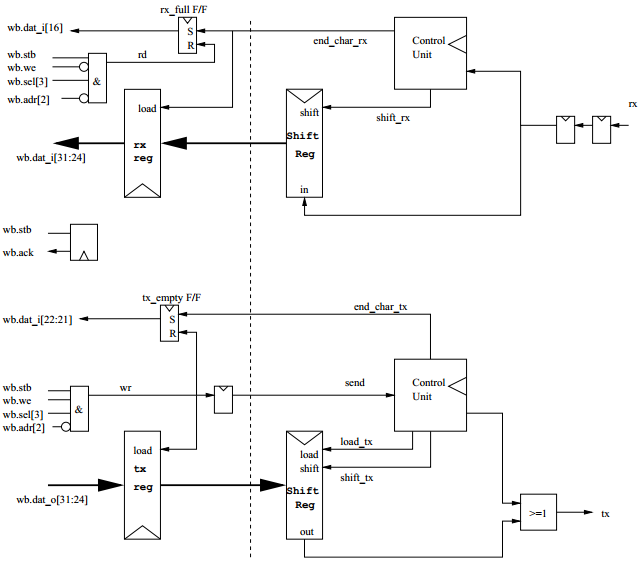
\includegraphics[scale=0.5]{blockdiagram.png}
\caption{The block diagram of our architecture}
\label{fig:block diagram}
\end{figure}

\subsection{How we tested our implementation}

First we simulated our design with a test bench and when that was
validated we tested our design by running a test program given to us
called dctsw.c. The input we gave was a 64 long array, with the numbers
1-64. We took these because we knew what the output of this would be.
The result is given at the home page.

\subsection{result of the interface implementation}
The following shows the result when a is [1 2 3 4 ... 63 64] as input to the DCT.
a=  \newline  \newline
\begin{tabular}{l l l l l l l l}
1 & 2 & 3 & 4 & 5 & 6 & 7 & 8 \\
9  &  10  &  11   & 12 &   13  &  14 &   15 &   16  \\
17   & 18  &  19  &  20  &  21  &  22  &  23  &  24  \\
25  &  26  &  27  &  28  &  29  &  30  &  31  &  32  \\
33  &  34  &  35  &  36  &  37  &  38  &  39  &  40  \\
41  &  42  &  43  &  44  &  45  &  46  &  47  &  48  \\
49  &  50  &  51  &  52  &  53  &  54 &   55  &  56  \\
57   & 58  &  59  &  60  &  61 &   62  &  63  &  64  \\
\end{tabular}
 \newline  \newline  \newline
8xDCT[a-128]=  \newline  \newline
\begin{tabular}{l l l l l l l l}
-6112  & -152   &   0   & -16   &   0  &   -8   &   0  &   -8 \\
-1167   &   0    &  0   &   0   &   0   &   0   &   0  &    0 \\
    0   &   0   &   0   &   0    &  0   &   0    &  0   &   0 \\
 -122  &    0   &   0   &   0   &   0   &   0    &  0   &   0 \\
    0    &  0   &   0   &   0    &  0   &   0    &  0   &   0 \\
  -37   &   0   &   0   &   0   &   0   &   0   &   0   &   0 \\
    0   &   0   &   0   &   0  &    0   &   0   &   0   &   0 \\
  -10   &   0   &   0  &    0   &   0   &   0   &   0   &   0 \\

\end{tabular}
 \newline  \newline  \newline
RND(8xDCT[a-128]/(8xQx1/2)) =  \newline  \newline
\begin{tabular}{l l l l l l l l}
  -96   &  -3   &   0   &   0  &    0  &    0   &   0 &     0 \\
  -24    &  0    &  0   &   0   &   0   &   0   &   0   &   0 \\
    0    &  0   &   0   &   0   &   0   &   0    &  0   &   0 \\
   -2    &  0   &   0    &  0   &   0   &   0    &  0   &   0 \\
    0    &  0    &  0    &  0   &   0   &   0  &    0   &   0 \\
    0    &  0   &   0    &  0   &   0   &   0    &  0    &   0 \\
    0    &  0   &   0    &  0   &   0   &   0    &  0     & 0 \\
    0    &  0   &   0   &   0   &   0   &   0   &   0     & 0 \\

\end{tabular}


\section{Performance counter}

In this lab we also implemented four performance counters that are
measuring the traffic on the WB. There are two counters that are
counting the number of m0.ack and m1.ack we get on WB and two counters
are counting how many (m0.ack and m0.stb) and (m1.ack and m1.stb) we get
on the bus. These counters are saved at address x’99000000, x’99000004,
x’99000008 and x’9900000C respectively in the memory.

We looked at these addresses when running the test program with
different cache settings. We ran it without any caches selected, with
I-cache selected, with D-cache selected and with both selected.  We saw
that the performance was increasing with the caches selected i.e. the
counters value decreased when caches were used i.e. there was less data
traffic on the wishbone bus. We got the best result when both caches
were selected. We did three runs with all the alternatives


\subsection{Result of performance counter}

ICache enabled and DCache enabled \newline
Clk cycles for ctr1: 797, ctr2: 155, ctr3: 964, ctr4: 271  \newline
Clk cycles for ctr1: 367, ctr2:  76, ctr3: 480, ctr4: 159 \newline
Clk cycles for ctr1: 367, ctr2:  76, ctr3: 480, ctr4: 159 \newline  \newline

ICache enabled and DCache disabled  \newline
Clk cycles for ctr1: 802, ctr2: 162, ctr3: 989, ctr4: 309  \newline
Clk cycles for ctr1: 447, ctr2:  80, ctr3: 954, ctr4: 309  \newline
Clk cycles for ctr1: 446, ctr2:  80, ctr3: 955, ctr4: 309  \newline  \newline

ICache disabled and DCache enabled \newline
Clk cycles for ctr1: 8639, ctr2: 1764, ctr3: 2254, ctr4: 270 \newline
Clk cycles for ctr1: 7887, ctr2: 1748, ctr3: 1127, ctr4: 158 \newline
Clk cycles for ctr1: 7887, ctr2: 1748, ctr3: 1127, ctr4: 158 \newline \newline

ICache disabled and DCache disabled \newline
Clk cycles for ctr1: 8728, ctr2: 1751, ctr3: 2533, ctr4: 309 \newline
Clk cycles for ctr1: 8728, ctr2: 1751, ctr3: 2533, ctr4: 309 \newline
Clk cycles for ctr1: 8728, ctr2: 1751, ctr3: 2533, ctr4: 309 \newline

\section{Conclusion}

In this lab we learned how to implement an interface to the wishbone bus
and performance counters that measured the data traffic on the wishbone
bus.  We tested the interface with both a test bench and given test
program called dctsw, with the image [1 2 3 4 … 63 64]. When we
validated the result, we created performance counters to count the
amount of traffic we got on the bus with different cache settings. We
saw that if we had no caches selected we got high traffic on the bus.
When we had one cache selected the traffic on the bus decreased. We saw
that when we enabled the I-cache the perforamance increased (avservärt)
compared to when the D-cache was enabled. The best result (least amount
of traffic) we got when we had both D-cache and I-cache was selected.


\section{Files}
\begin{itemize}
	\item [lab1uarttop.sv] In this file we implemented our interface between the WB and the UART.
	\item [perftop.sv] In this file we implemented our performance counter.
	\item [uarttb.sv] In this file we tested our hardware.
	\item [dctsw.c] In this file we ran a software DCT to measure the traffic on the wish bone bus.
\end{itemize}



\newpage
\begin{appendices}
\begin{changemargin}{-3cm}{-3cm}

\section{lab1uarttop.sv}
\lstinputlisting[language=Verilog,caption={Code lab1uarttop},label=lab1uarttop]{lab1uarttop.sv}
\newpage
\section{perftop.sv}
\lstinputlisting[language=Verilog,caption={Code perftop},label=perftop]{perftop.sv}
\newpage
\section{uarttb.sv}
\lstinputlisting[language=Verilog,caption={Code uarttb},label=uarttb]{uarttb.sv}
\newpage
\section{dctsw.c}
\lstinputlisting[language=Verilog,caption={Code dctsw},label=dctsw]{dctsw.c}
\end{changemargin}
\end{appendices}

\end{document}
